% !TeX root = ../libro.tex
% !TeX encoding = utf8

\setchapterpreamble[c][0.75\linewidth]{%
	\sffamily
	% Introducción al capitulo
	\par\bigskip
}
\chapter{Teoría de Grafos}\label{ch:segundo-capitulo}
Las definiciones y conceptos de este capítulo han sido extraídos de libros~\cite{algorithms}.

\section{Conceptos básicos y propiedades asociadas a grafos}
Vamos a comenzar viendo algunas definiciones y conceptos básicos.

\begin{definicion}
	Un \textit{grafo no  dirigido} es un par (\textbf{V}, \textbf{E}), donde \textbf{V} es un conjunto no vacío, a cuyos elementos denominaremos \textit{vértices} o \textit{nodos}, y \textbf{E} es un conjunto finito de pares de elementos de \textbf{V}, a los que llamaremos \textit{aristas} o \textit{lados}.
\end{definicion}

\begin{itemize}
	\item A los nodos $v_1$ y $v_2$ que forman una arista $e=\{v_1, v_2\}$ se les llama \textit{extremos} de $e$. Cuando esto ocurra, se dirá que los vértices $v_1$ y $v_2$ son \textit{adyacentes} o \textit{vecinos}.
	
	\item Se dirá que una arista $e$ es \textit{incidente} con un vértice $v$ cuando $v$ sea uno de sus extremos. En dicho caso se dirá que $e$ \textit{incide} en $v$.
\end{itemize}

\begin{definicion}
	Se denominará \textit{grado de incidencia} de un vértice $v\in V$ (que denotaremos por $g(v)$), al número de aristas incidentes con $v$.
\end{definicion}

Por conveniencia, no consideraremos lados que conecten un vértice consigo mismo, es decir, lados del tipo $\{v, v\}$. \\

En este tipo de grafos no se tiene en cuenta el orden en el que aparecen los vértices en una arista, es decir,  $e=\{v_1, v_2\}=\{v_2, v_1\}$. El siguiente tipo de grafo sí que diferencia entre ambas aristas, incluyendo una orientación sobre las mismas.

\begin{definicion}
	Un \textit{grafo dirigido} es un grafo $G$ cuyas aristas cuentan con una orientación, en este caso pasarán a ser llamadas \textit{arcos}. En este caso denotaremos los arcos como $e=(v_1,v_2)$, siendo $e$ un arco orientado de $v_1$ hacia $v_2$.
\end{definicion}

Cuando planteamos un grafo asociado a un problema, las aristas suelen ser caminos entre nodos, con un coste asociado, para introducir estos costes definimos el siguiente tipo de grafo.

\begin{definicion}
	Un \textit{grafo ponderado} (o grafo con pesos), es una terna $(V,E,\omega)$ donde el par $(V,E)$ representa un grafo (dirigido o no dirigido), y $\omega:E\rightarrow\mathbb{R}$ es una aplicación que asigna a cada arista o arco el peso asociado.
\end{definicion}

En la \autoref{fig:graf-ej} podemos observar ejemplos de las definiciones anteriores, por ejemplo, los vértices $0$ y $2$ son adyacentes, y el grado de incidencia del vértice $a$ es $4$. \\

\begin{figure}[htb]
	\centering
	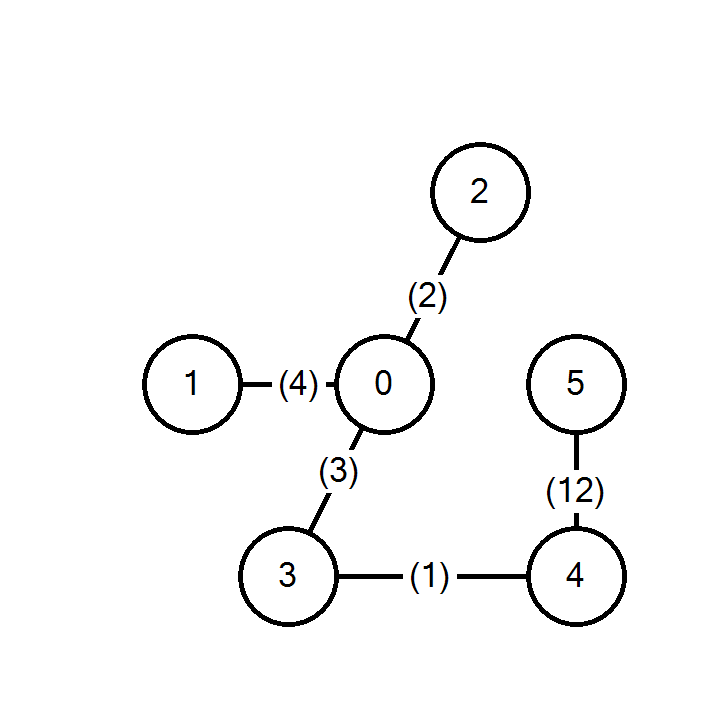
\includegraphics[width=0.4\linewidth]{graf-ej-1}
	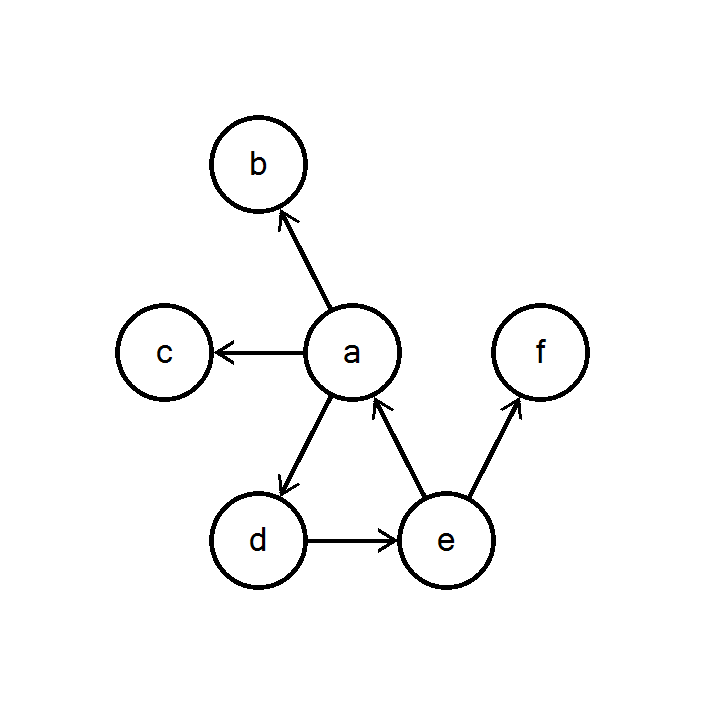
\includegraphics[width=0.4\linewidth]{graf-ej-2}
	\caption{Ejemplo de grafo no dirigido ponderado, izquierda, y grafo dirigido no ponderado, derecha.}
	\label{fig:graf-ej}
\end{figure}

A continuación plantearemos algunas definiciones sobre distintos tipos de grafos.

\begin{definicion}
	Un \textit{grafo finito} es un grafo $G$ (dirigido o no dirigido), con un número finito de vértices, es decir, el conjunto $V$ es finito.
\end{definicion}

\begin{definicion}
	Un \textit{grafo de incidencia finita} es un grafo $G$ donde el grado de incidencia de cada vértice es finito, es decir, $g(v)$ es finito para cada $v\in V$.
\end{definicion}

\begin{definicion}
	Dado un grafo $G=(V,E)$: 
	\begin{itemize}
		\item Se dirá que $G'=(V',E')$ es un \textit{subgrafo} de $G$ si $V'\subseteq V$ y $E'\subseteq E$.
		\item Se dirá que $G'=(V,E')$ es un \textit{subgrafo parcial} de $G$ si $E'\subseteq E$.
	\end{itemize} 
\end{definicion}

\begin{definicion}
	Dado un grafo $G=(V,E)$ y $B\subseteq V$, se dirá \textit{subgrafo de G inducido por B} a $G_B=(B,E_B)$ con
	$$E_B=\{(i,j)\in E:\ i,j\in B\}\ |\ E_B=\{\{i,j\}\in E:\ i,j\in B\}$$
\end{definicion}

Un concepto natural que surge al hablar de grafos es el de camino entre dos nodos, definimos a continuación formalmente el concepto tanto del camino como tal como de la longitud del mismo.

\begin{definicion}
	Dado un grafo $G$, un \textit{camino} es una sucesión de vértices $v_1v_2...v_{n+1}$ y aristas $e_1e_2...e_n$ tal que $e_i=\{v_i,v_{i+1}\}$ si es un grafo no dirigido, o bien $e_i=(v_i,v_{i+1})$ si es un grafo dirigido, $\forall i \in \{1,...,n\}$. Para referirnos a un camino de ahora en adelante, utilizaremos la sucesión de vértices $v_1...v_{n+1}$ si no es necesario conocer las aristas en concreto, o $e_1...e_n$ si necesitamos conocerlas.
\end{definicion}

\begin{definicion}
	Se define la \textit{longitud} de un camino $v_1v_2...v_{n+1}$ con aristas $e_1e_2...e_n$ como sigue: 
	$$Long(v_1v_2...v_{n+1}) = \sum_{i=1}^{n}\omega(e_i)$$
	En caso de que no sea un grafo ponderado, supondremos coste $1$ para todas las aristas, en cuyo caso, la longitud del camino será $n$.
\end{definicion}

Definimos a continuación una función que nos será útil más adelante.

\begin{definicion}
	Dado un grafo finito $G=(V,E)$ y $v_0,v_1\in V$, Definimos $d:V\times V \rightarrow \mathbb{R}\cup \{\infty\}$ como sigue:
	$$d(v_0,v_1)= \left\{ \begin{array}{lcc}
		min\{Long(v_0...v_1) : v_0...v_1\ camino\ desde\ v_0\ a\ v_1\} &   si\ existe\ camino\ entre\ v_0\ y\ v_1 \\
		\\ \infty &  en\ otro\ caso
	\end{array}
	\right.$$
\end{definicion}

Sabemos que existe el mínimo, pues, como los conjuntos de vértices y aristas son finitos, el conjunto de caminos entre dos vértices es también finito.

Probaremos a continuación que, tal y como sugiere la definición, $d$ es un distancia.

\begin{proposicion}\label{prop:distancia}
	Sea $G$ un grafo finito no dirigido, no ponderado o ponderado con pesos exclusivamente positivos, se verifica que $d:V\times V \rightarrow \mathbb{R}$ con la definición anterior es una distancia en $G$.
\end{proposicion}

\begin{proof}
	Dado que los únicos caminos de longitud $0$ son aquellos en los que no hay aristas, es claro que $d(v_0, v_1) = 0 \Leftrightarrow v_0 = v_1$. La simetría es clara, pues, en un grafo no dirigido, un camino desde $v_0$ a $v_1$ es también un camino desde $v_1$ a $v_0$, dado que podemos recorrer las aristas en los dos sentidos. Para probar la desigualdad triangular, es decir, $\forall v_0, v_1, v_2 \in V,\ d(v_0,v_1) \leq d(v_0,v_2) + d(v_2,v_1)$, hay que distinguir dos casos, el primero, si no existe ningún camino que conecte $v_0$ con $v_2$ o ningún camino que conecte $v_2$ con $v_1$, en cuyo caso se tendría $d(v_0,v_1)\leq \infty$, por lo que siempre se verifica la desigualdad. En caso contrario, si existieran caminos $c_1$ y $c_2$ que conectan $v_0$ con $v_2$ y $v_2$ con $v_1$, respectivamente, $d(v_0,v_1)\leq Long(c) = Long(c_1) + Long(c_2)$, donde $c$ es el camino que resulta de unir $c_1$ y $c_2$, esta última desigualdad es cierta por la definición de $d$, para cualquier par de caminos $c_1$, $c_2$, por lo que, tomando ínfimos sobre estos caminos, obtenemos que $d(v_0,v_1) \leq d(v_0,v_2) + d(v_2,v_1)$, como se quería.
\end{proof}

\begin{proposicion}
	Sea $G$ un grafo dirigido, no ponderado o ponderado con pesos exclusivamente positivos, se verifica que $d:V\times V \rightarrow \mathbb{R}$ con la definición anterior es una distancia asimétrica en $G$.
\end{proposicion}

Esta proposición no necesita demostración, pues los argumentos utilizados para probar la no negatividad y la desigualdad triangular en la \autoref{prop:distancia} son válidos también para grafos dirigidos.

\begin{definicion}
	Dado un grafo $G=(V,E)$ y un camino $v_0...v_1$ entre los vértices $v_0$ y $v_1$, a dicho camino se le llama \textit{camino de longitud mínima} desde $v_0$ a $v_1$ si y solo si es la geodésica entre $v_0$ y $v_1$, es decir:
	$$Long(v_0...v_1) = d(v_0, v_1)$$
\end{definicion}

Nótese que en el grafo, las líneas entre puntos son caminos entre vértices. Veremos a continuación un par de propiedades muy interesantes asociadas a este tipo de caminos.

\begin{proposicion}
	Dado un camino de longitud mínima $v_0...v_i...v_1$ desde $v_0$ a $v_1$, se verifica:
	\begin{itemize}
		\item $v_0...v_i$ es un camino de longitud mínima desde $v_0$ a $v_i$.
		\item $v_i...v_1$ es un camino de longitud mínima desde $v_i$ a $v_1$.
	\end{itemize}
\end{proposicion}

\begin{proof}
	Sea $e_1...e_{i-1}$ el conjunto de aristas asociadas al camino entre $v_0$ y $v_i$, entonces, por contradicción, supongamos que $v_0...v_i$ no es un camino de longitud mínima (el caso en que $v_i...v_1$ no es un camino de longitud mínima es análogo), al no ser camino de longitud mínima, debe existir otro camino entre $v_0$ y $v_i$ de longitud menor, es decir, $\exists e_1'...e_m'$ camino entre $v_0$ y $v_i$ con $Long(e_1'...e_m') < Long(e_1...e_{i-1})$. Llamemos $e_i...e_n$ al conjunto de aristas del camino entre $v_i$ y $v_1$, entonces, juntando el nuevo camino entre $v_0$ y $v_i$ con éste último, obtenemos:
	\begin{equation}
		\begin{split}
			Long(e_1'...e_m'e_i...e_n) & =Long(e_1'...e_m') + Long(e_i...e_n) \\
			& < Long(e_1...e_{i-1}) + Long(e_i...e_n) \\
			& =	Long(e_1...e_n)
		\end{split}
	\end{equation}
	Esto es una contradicción pues, por hipótesis, $Long(e_1...e_n) = d(v_0,v_1)$, al ser $e_1...e_n$ camino de longitud mínima, pero hemos encontrado entonces un camino entre $v_0$ y $v_1$, el cual es $e_1'...e_m'e_i...e_n$, de longitud menor, lo que no puede ser.
\end{proof}

\begin{proposicion}
	Sea $G=(V,E,\omega)$ un grafo de incidencia finita ponderado con pesos positivos tal que:
	\begin{itemize}
		\item $\omega (e)\geq a>0\ \ \ \forall e\in E.$
	\end{itemize}
	Entonces, si existe un camino entre dos nodos, existe un camino de longitud mínima entre ambos (geodésica).
\end{proposicion}

\begin{proof}
	Sean $v_0,v_1\in V$ tales que existe un camino de longitud $L>0$ entre ambos, si $c$ es otro camino entre $v_0$ y $v_1$ de $K$ aristas, entonces
	$$Long(c) \geq Ka$$
	por hipótesis.\\
	Si $Ka>L$, $c$ no puede ser una geodésica, consideramos entonces el subgrafo inducido por los vértices que se pueden unir con $v_0$ mediante caminos de $K\leq \frac{L}{a}$ lados. El vértice $v_1$ pertenece a dicho grafo por el camino inicial. Ahora, por ser $G$ un grafo de incidencia finita, se tiene que dicho subgrafo es finito y, por tanto, existe una geodésica que une $v_0$ con $v_1$ en el subgrafo y, dado que el resto de caminos $c$ entre $v_0$ y $v_1$ tienen longitud $Long(c) > L$, la geodésica en el subgrafo es geodésica también en G.
\end{proof}

Para trabajar con grafos, necesitamos representarlos de alguna manera, para ello se definen a continuación dos estructuras muy utilizadas a la hora de la representación de grafos:

\begin{definicion}
	Dado un grafo finito $G$, con $|V|=n$, llamaremos \textit{matriz de adyacencia} de $G$ a una matriz $A_{n\times n}=(a_{ij})$ de tal manera que:
	$$a_{ij}= \left\{ \begin{array}{lcc}
		1 &   si\ (v_i,v_j)\in E\ (\{v_i,v_j\}\ o\ \{v_j,v_i\}\in E) \\
		\\ 0 &  en\ otro\ caso
	\end{array}
	\right.$$
\end{definicion}

\begin{definicion}
	Dado un grafo finito $G$, con $|V|=n$, se define la \textit{lista de adyacencia} de $v \in V$ como:
	$$Adj(v) = \{u \in V : (v,u)\in E (\{v,u\}\ o\ \{u,v\}\in E)\}$$
	De tal manera que para representar el grafo, basta calcular la lista de adyacencia de cada vértice.
\end{definicion}



\endinput
